%%%%%%%%%%%%%%%%%%%%%%%%%%%%%%%%%%%%%%%%%%%%%%%%%%%%%%%%%%%%%%%%%%%%%
%
%  This is a sample LaTeX input file for your contribution to 
%  the MC2013 conference. Modified by R.C. Martineau at INL from A. 
%  Sood at LANL, from J. Wagner ORNL who obtained the original class 
%  file by Jim Warsa, LANL, 16 July 2002}
%
%  Please use it as a template for your full paper 
%    Accompanying/related file(s) include: 
%       1. Document class/format file: mc2013.cls
%       2. Sample Postscript Figure:   figure.eps
%       3. A PDF file showing the desired appearance: template.pdf 
%    Direct questions about these files to: richard.martinea@inl.gov
%
%    Notes: 
%      (1) You can use the "dvips" utility to convert .dvi 
%          files to PostScript.  Then, use either Acrobat 
%          Distiller or "ps2pdf" to convert to PDF format. 
%      (2) Different versions of LaTeX have been observed to 
%          shift the page down, causing improper margins.
%          If this occurs, adjust the "topmargin" value in the
%          mc2013.cls file to achieve the proper margins. 
%
%%%%%%%%%%%%%%%%%%%%%%%%%%%%%%%%%%%%%%%%%%%%%%%%%%%%%%%%%%%%%%%%%%%%%


%%%%%%%%%%%%%%%%%%%%%%%%%%%%%%%%%%%%%%%%%%%%%%%%%%%%%%%%%%%%%%%%%%%%%
\documentclass{mc2013}
%
%  various packages that you may wish to activate for usage 
\usepackage{graphicx}
\usepackage{tabls}
\usepackage{afterpage}
\usepackage{cites}
\usepackage{amsmath}
\usepackage{amssymb}
\usepackage{listings}
%\usepackage{epsf}
%
%
% Insert authors' names and short version of title in lines below
%
\newcommand{\authorHead}      % Author's names here
   {A.Alfonsi, C. Rabiti, D. Mandelli, J.J. Cogliati, R.A. Kinoshita}  
\newcommand{\shortTitle}      % Short title here
   {Short version of title as entered by author on web page}  
%%%%%%%%%%%%%%%%%%%%%%%%%%%%%%%%%%%%%%%%%%%%%%%%%%%%%%%%%%%%%%%%%%%%%
%
%   BEGIN DOCUMENT
%
%%%%%%%%%%%%%%%%%%%%%%%%%%%%%%%%%%%%%%%%%%%%%%%%%%%%%%%%%%%%%%%%%%%%%
\begin{document}

%
%      Headers and Footers
\afterpage{%
\fancyhf{}%
\fancyhead[CE]{              
{\scriptsize \authorHead}}                                                
\fancyhead[CO]{               
{\scriptsize \shortTitle}}                  
%\lfoot{\scriptsize{
%International Conference on Mathematics and Computational Methods
%Applied to Nuclear Science \& Engineering (M\&C 2013), 
%\\ Sun Valley, Idaho, USA, May 5-9, 2013.}}%
\rfoot{\thepage/\totalpages{}}%

\pagestyle{fancy}
%\setlength{\topmargin}{-20pt}
}
 
\normalsize

%\setlength{\baselineskip}{16.8pt}
\vspace{-3pt}

% 
% TITLE
%

\begin{center}
\textbf{\large \\%
TITLE OF THE PAPER 
}
% 
% FIRST AUTHORS 
%
\\
\setlength{\baselineskip}{14pt}
\textbf{A. Alfonsi, C. Rabiti, D. Mandelli, J.J. Cogliati, R.A. Kinoshita} \\ %\footnote{Footnote, if necessary, in Times New Roman font and font size 9} 
Idaho National Laboratory  \\
2525 Fremont Avenue, Idaho Falls, ID 83415 \\
\{andrea.alfonsi, cristian.rabiti, diego.mandelli, joshua.cogliati, robert.kinoshita\}@inl.gov \\

\end{center}

%
% SET RAGGED RIGHT MARGIN
%
\raggedright


\section*{ABSTRACT} 
\begin{quote}
\begin{small}
To be added

\emph{Key Words}: Reactor Simulation, Probabilistic Risk Assessment, Dynamic PRA, Monte-Carlo, Relap-7 %, Three Miles Island, 
\end{small} 
\end{quote}

\setlength{\baselineskip}{14pt}
\normalsize

%%%%%%%%%%%%%%%%%%
\Section{INTRODUCTION} 
%%%%%%%%%%%%%%%%%%


RAVEN (\textbf{R}eactor \textbf{A}nalysis and \textbf{V}irtual control \textbf{EN}viroment) is a complex software tool that acts as the control logic driver for RELAP-7. The goal of this paper is to highlight the software structure of the code and its utilization in conjunction with the newly developed Thermo-Hydraylic code RELAP-7. RAVEN is a software framework that allows dispatching the following functionalities:
\begin{itemize}
\item Derive and actuate the control logic required to:
\begin{itemize}
\item Simulate the plant control system;
\item Simulate the operator actions (guided procedures);
\item Perform Monte-Carlo sampling of random distributed events;
\item Perform event tree based analysis.
\end{itemize}
\item Provide a Graphical User Interface (GUI) to:
\begin{itemize}
\item Input a plant description to RELAP-7(components, controlled variables, controlled
parameters);
\item Concurrent monitoring of Controlled Parameters;
\item Concurrent alteration of Controlled Parameters.
\end{itemize}
\item Provide a post-processing data mining capability based on:
\begin{itemize}
\item Dimensionality reduction;
\item Cardinality reduction.
\end{itemize}
\end{itemize}
The paper is divided in three main sections:
\begin{itemize}
\item RAVEN mathematical framework;
\item RAVEN software structure;
\item Demonstration of a Station Black Out (SBO) analysis of a Pressurized Water Reactor (PWR).
\end{itemize}

%%%%%%%%%%%%%%%%%%%%%%%%%%%%
\Section{MATHEMATICAL FRAMEWORK}
%%%%%%%%%%%%%%%%%%%%%%%%%%%%
\label{sec:mathFramework}

In the following paragraphs the mathematical framework is briefly described, analyzing the set of the
equations needed to model the control system in a nuclear power plant.

\Subsection{Plant and Control System Model} 
\label{sec:PlantControlModel}
The first step will be the derivation of the mathematical model representing, at a high level of abstraction,
the plant and control system model. Let be $\bar{\theta}(t)$ a vector describing the plant status in the phase space, and the governing equation:
\begin{equation}
\frac{\partial \bar{\theta}}{\partial t} = \bar{H}(\theta(t),t)
\label{eq:SystemDynamics}
\end{equation}
In the above equation we have assumed the time differentiability in the phase space. This is in generally
not required and it is abused here for compactness of the notation. Now an arbitrary decomposition of the
phase space is performed:
\begin{equation}
\bar{\theta}=\binom{\bar{x}}{\bar{v}}
\label{eq:firstDecomposition}
\end{equation}
The decomposition is made in such a way that $x$ represent the unknowns solved by RELAP-7, while $v$ are the variables directly controlled by the control system . The governing equation is now casted in a system of equations:
\begin{equation}
\begin{cases} 
\dfrac{\partial \bar{x}}{\partial t} = \bar{F}(\bar{x},\bar{v},t) \\ 
\dfrac{\partial \bar{v}}{\partial t} = \bar{V}(\bar{x},\bar{v},t) \\
\end{cases}
\label{eq:generalSystemEquation}
\end{equation}
As a consequence of this splitting, the contains components state variables of the phase space now that
are continuous while contains all variables describing the discrete state variables that are of the system
usually handled by the control system. As a next step, we realize that the function 
$\bar{V}(\bar{x},\bar{v},t)$ 
representing the control system, does not depend on the knowledge of the complete status of the system but on a restricted subset that we call control variables $\bar{C}$:
\begin{equation}
\begin{cases} 
\dfrac{\partial \bar{x}}{\partial t} = \bar{F}(\bar{x},\bar{v},t) \\
\bar{C} = \bar{G}(\bar{x},t) \\ 
\dfrac{\partial \bar{v}}{\partial t} = \bar{V}(\bar{x},\bar{v},t) 
\end{cases}
\label{eq:generalSystemEquationwithControl}
\end{equation}
where 
$\bar{C}$
is a vector which having lesser dimensionality than
$\bar{x}$
and therefore is more convenient to work with. In rest of this document the following naming will be adopted: $\bar{C}$: monitored variables $\bar{v}$:
controlled variables.
Note that even if it seems more appropriate, the standard naming of signals (monitored)
and status (controlled) is not yet used. The reason for this choice is that, the chosen naming better mirrors
the computational pattern between RAVEN and RELAP 7 and moreover the definition of signals is more
tight to the definition of the control logic for each component and therefore relative rather than absolute in
the overall system analysis. In fact we could have signal for a component that are status of another creating
a definition that would be not unique. Another reason is that the standard naming will loose every meaning
once used also for uncertainty analysis.

%%%%%%%%%%%%%%%%%%%%%%%%%%%%%%
\Subsection{Operator Splitting Approach} 
%%%%%%%%%%%%%%%%%%%%%%%%%%%%%%
\label{sec:operatorSplitting}

System of equations shown in Eq.~\ref{eq:generalSystemEquationwithControl} is, generally speaking, fully coupled and in the past it has always been solved following an operator splitting approach. The reasons for this choice are several:
\begin{itemize}
\item Control system reacts with an intrinsic delay anyhow;
\item The reaction of the control system might move the system between two different discrete state and
therefore numerical errors will be always of first order unless the discontinuity will be treated explicitly.
\end{itemize}
RAVEN is, thus, using this approach. Therefore Eq.~\ref{eq:generalSystemEquationwithControl} becomes:
\begin{equation}
\begin{cases} 
\dfrac{\partial \bar{x}}{\partial t} = \bar{F}(\bar{x},\bar{v}_{t_{i}-1},t) \\
\bar{C} = \bar{G}(\bar{x},t) \\ 
\dfrac{\partial \bar{v}}{\partial t} = \bar{V}(\bar{x},\bar{v}_{t_{i}-1},t) 
\end{cases}
\label{eq:generalSystemEquationwithControlSplitting}
\end{equation}

%%%%%%%%%%%%%%%%%%%%%%%%%%%%%%
\Subsection{The auxiliary plant and component status variables.} 
%%%%%%%%%%%%%%%%%%%%%%%%%%%%%%
\label{sec:auxiliary}
So far it has been assumed that all information needed are contained in $\bar{x}$ and $\bar{v}$. Even if, as previously shown, these information are sufficient for the calculation of the system status in every point in time, it is not a practical and efficient way to implement the control system.
In order to facilitate the implementation of the control logic, it's been implemented a system of auxiliary variables.
The auxiliary variables are those that in statistical analysis are artificially added to non-Markovian system into the space phase to obtain back a Markovian behavior, so that only the previous time step information are needed to determine the future status of the system
These variables can be classified into two types: 
\begin{itemize}
\item Global status auxiliary control variables: scram signal, time at which scram event begins, hot shut down, time at which hot shut down event begins, cold shut down, etc.;
\item Component status auxiliary variables like: correct operating status, time from abnormal event, etc.
\end{itemize}
Thus, the introduction of the auxiliary system into the mathematical framework leads to the following formulation of the Eq.~\ref{eq:generalSystemEquationwithControlSplitting}:
\begin{equation}
\begin{cases} 
\dfrac{\partial \bar{x}}{\partial t} = \bar{F}(\bar{x},\bar{v}_{t_{i}-1},t) \\
\bar{C} = \bar{G}(\bar{x},t) \\ 
\dfrac{\partial \bar{a}}{\partial t} = \bar{A}(\bar{x},\bar{C},\bar{a},\bar{v}_{t_{i}-1},t) \\
\dfrac{\partial \bar{v}}{\partial t} = \bar{V}(\bar{x},\bar{v}_{t_{i}-1},t) 
\end{cases}
\label{eq:generalSystemEquationwithControlSplittingAndAux}
\end{equation}
%%%%%%%%%%%%%%%%%%%%%%%%
\Section{SOFTWARE STRUCTURE} 
%%%%%%%%%%%%%%%%%%%%%%%%
\label{sec:softwareStructure}
RAVEN is a C++/Python software, coded in an high modular and object-oriented way and based on two software sections:
\begin{itemize}
\item MOOSE(\textbf{M}ultiphysics \textbf{O}bject-\textbf{O}riented \textbf{S}imulation \textbf{E}nviroment);
\item RELAP-7.
\end{itemize}
%%%%%%%%%%%%%%%%%%%%%%%%%%%%%%
\Subsection{MOOSE/RELAP-7.} 
%%%%%%%%%%%%%%%%%%%%%%%%%%%%%%
MOOSE is a computer simulation framework,  developed at Idaho National Laboratory (INL), that simplifies the process for predicting the behavior of complex systems and developing non-linear, multiphysics simulation tools. As opposed to traditional data-flow oriented computational frameworks, MOOSE is founded on the mathematical principle of Jacobian-free Newton-Krylov (JFNK) solution methods. Utilizing the mathematical structure present in JFNK, physics are modularized into “Kernels” allowing for rapid production of new simulation tools. In addition, systems are solved fully coupled and fully implicit employing physics based preconditioning which allows for great flexibility even with large variance in time scales. In addition to provide the algorithms for the solution of the differential equation, MOOSE also provides all the manipulation tools for the C++ classes containing the solution vector. This framework has been used to construct and develop the Thermo-Hydraylic code RELAP-7, giving a enormous flexibility in the coupling procedure with RAVEN.
RELAP-7 is the next generation nuclear reactor system safety analysis. It will become the main reactor systems simulation toolkit for RISMC (\textbf{R}isk \textbf{I}nformed \textbf{S}afety \textbf{M}argin \textbf{C}haracterization) and the next generation tool in the RELAP reactor safety/systems analysis application series (the replacement for RELAP5). The key to the success of RELAP-7 is the simultaneous advancement of physical models, numerical methods, and software design while maintaining a solid user perspective. Physical models include both PDEs (Partial Differential Equations) and ODEs (Ordinary Differential Equations) and experimental based closure models. RELAP-7 will eventually utilize well posed governing equations for multiphase flow, which can be strictly verified.RELAP-7 uses modern numerical methods, which allow implicit time integration, higher order schemes in both time and space, and strongly coupled multi-physics simulations.
RELAP-7 is the solver for the plant system except for the control system. From the mathematical
formulation presented so far, RELAP-7 solves 
$\frac{\partial \bar{x}}{\partial t} = \bar{F}(\bar{x},\bar{v}_{t_{i}-1},t)$.
\begin{figure}[h] 
  \centering
     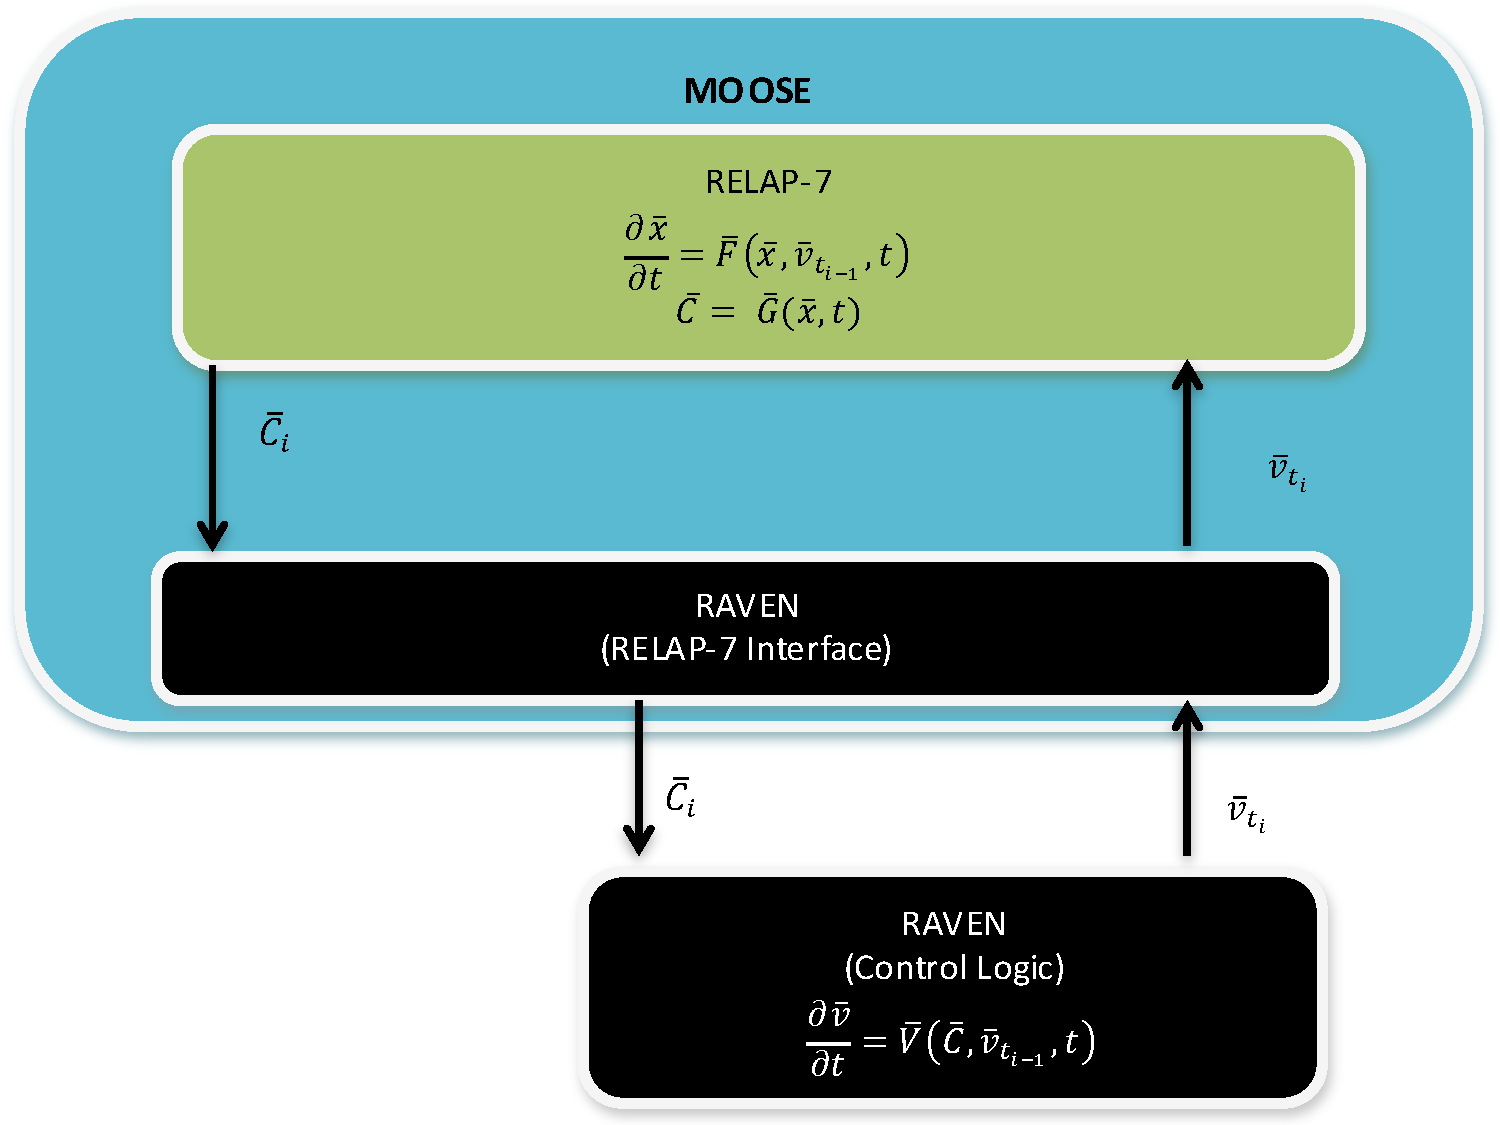
\includegraphics[width=0.5\textwidth]{figures/ControlSystemSoftwareLayout.pdf}
  \caption{Control System Software Layout.}
   \label{fig:ControlSoftwareLayout}
\end{figure}
The nuclear power plant is represented and modeled by a set of components (Pipes, Valves, Branches, etc.) and each component type corresponds to a C++ class.
%%%%%%%%%%%%%%%%%%%%%%%%%%%%%%
\Subsection{RAVEN .} 
%%%%%%%%%%%%%%%%%%%%%%%%%%%%%%
As briefly mentioned, RAVEN has been coded in high modular and pluggable way in order to make easier the integration of different program languages (C++, Python) and coupling with other applications based on MOOSE and not. The code is constituted by four modules:
\begin{itemize}
\item RAVEN/RELAP-7 interface;
\item Python Control Logic;
\item Python Calculation Driver;
\item Graphical User Interface (optional).
\end{itemize}

%%%%%%%%%%%%%%%%%%%%%%%%%%%%%%
\Subsubsection{RAVEN/RELAP-7 interface.} 
%%%%%%%%%%%%%%%%%%%%%%%%%%%%%%
The RAVEN/RELAP-7 interface, coded in C++, is the container of all the tools needed to interact with RELAP-7/MOOSE. It has been designed in order to be general and pluggable with differen solvers simultaneosly in order to allow an easier and faster development of the control logic/PRA capabilities for multi-physics applications.The interface provides all the capabilities to control, monitor, and process the parameters/quantities in order to drive the RELAP-7/MOOSE calculation. In addiction, it contains the tools to comunicate to the general MOOSE input parser which information, i.e. input syntax, must be inputted in order to run a RAVEN driven calculation. It includes four main sections so far:
\begin{itemize}
\item RavenMonitored class;
\item RavenControlled class;
\item RavenAuxiliary class;
\item RavenDistributions class.
\end{itemize}
%%%
% Monitored
%%%
The RavenMonitored class provides the connection with the calculation framework in order to retrieve the post-processed quantities from the simulation (i.e. average fuel temperature, average fluid pressure in a component, etc.). The typical input structure for a Monitored parameter in RAVEN is as following:
\begin{lstlisting}
[Monitored]
  [./MaxTempCladCH1]
    component_name = CH1
    operator = NodalMaxValue
    path = CLAD:TEMPERATURE
    data_type = double
  [../]
  [./MaxTempCladCH2]
    component_name = CH2
    operator = NodalMaxValue
    path = CLAD:TEMPERATURE
    data_type = double
  [../]

  ...

[]
\end{lstlisting}
Whithin the block identified by the keyword \textbf{Monitored}, the user can specify the monitored quantities must be processed during the calculation. Each monitored variable is identified through a \textbf{Raven Alias} (i.e. MaxTempCladCH1), the name that is used in the control logic python input in order to refer to the parameter contained in the simulation.
The user has to provide different information in order to build a monitored variable:
\begin{itemize}
  \item \textbf{component\_name}, the name of the RELAP-7 component that contains the variable the code must act on;
  \item \textbf{operator}, the post-processor oparation that must be performed on the variable;
  \item \textbf{path}, the variable name and its location within the calculation framework (RELAP-7/MOOSE variable name);
  \item \textbf{data\_type}, data type (i.e. double, float, int, bool).
\end{itemize}
RAVEN can use all the post-processor operators that are available in MOOSE [reference] (i.e. ElementAverageValue, NodalMaxValue, etc.). Depending on which component it's acting on, some operations may be disabled (i.e. ElementAverageValue is not available in 0-D components).
%%%
% Controlled
%%%
\\The RavenControlled class provides the link between RAVEN and RELAP-7/MOOSE in order to retrieve and/or change properties within the simulation (i.e. fuel thermal conductivity, pump mass flow, etc.). The typical input structure for a Controlled parameter in RAVEN is as following:
\begin{lstlisting}
[Controlled]
  control_logic_input = control_logic_input_file_name
  [./power_fraction_CH1]
    property_name = FUEL:power_fraction
    data_type = double
    component_name = CH1
  [../]
  [./power_fraction_CH2]
    property_name = FUEL:power_fraction
    data_type = double
    component_name = CH2
  [../]

  ...

[]
\end{lstlisting}
Inwardly the block identified by the keyword \textbf{Controlled}, the user can specify the properties that, during the calculation, will be controlled through the Python control logic. The name and path of the control logic input file are provided by the parameter  \textbf{control\_logic\_input} (not specifying the ".py" extension). Each controlled variable is identified through a \textbf{Raven Alias} (i.e. power\_fraction\_CH1), the name that is used in the control logic python input in order to refer to the parameter contained in the simulation.
The user has to provide different information in order to build a controlled variable:
\begin{itemize}
  \item \textbf{component\_name}, the name of the RELAP-7 component that contains the variable the code must act on;
  \item \textbf{property\_name}, the variable name and its location within the calculation framework (RELAP-7/MOOSE variable name);
  \item \textbf{data\_type}, data type (i.e. double, float, int, bool).
\end{itemize}
Through this class, RAVEN is able to retrieve property values and, in case of changes, push the new values back into the simulation. 
%%%
% Auxiliary
%%%
\\The RavenAuxiliary class is the container of auxiliary variables. The Raven Auxiliary system is not connected with RELAP-7/MOOSE enviroment. The typical input structure for a auxiliary parameter in RAVEN is as following:
\begin{lstlisting}
[RavenAuxiliary]
  [./scram_start_time]
    data_type     = double
    initial_value = 61.0
  [../]
  [./CladDamaged]
    data_type     = bool
    initial_value = False
  [../]
  
  ...

[]
\end{lstlisting}
Each auxiliary variable is identified through a \textbf{Raven Alias} (i.e. CladDamaged), the name that is used in the control logic python input in order to refer to the parameter contained in the RAVEN interface.
The user has to provide different information in order to build a auxiliary variable:
\begin{itemize}
  \item \textbf{initial\_value}, initialization value;
  \item \textbf{data\_type}, data type (i.e. double, float, int, bool).
\end{itemize}
As previously mentioned, these variables are needed to ensure that system remains Markovian, so that only the previous time step information are necessary to determine the future status of the plant. 
%%%
% Distributions
%%%
// The RavenDistributions class contains the algorithms, structures and interfaces for several predifined probability distributions. It is only available in the python control logic, since it is not needed a direct interaction with RAVEN/RELAP-7/MOOSE enviroment. The user can actually choose among nine different types of distribution (i.e. Normal, Triangular, Uniform, Exponential, etc.), each of them, in order to be intialized, requires a different set of parameters.
The following input, for example, builds a Normal and a Triangular distribution:
\begin{lstlisting}
[Distributions]
  [./ExampleNormalDis]
    type =  NormalDistribution
    mu = 1
    sigma = 0.01
    xMax = 0.8
    xMin = 0
  [../]
  [./ExampleTriangularDis]
    type   = TriangularDistribution
    xMin  = 1255.3722 
    xPeak = 1477.59
    xMax  = 1699.8167 
  [../]
  ...
[]
\end{lstlisting}
The class RavenDistributions is the base of the Monte-Carlo and Dynamic Event Tree capabilities present in RAVEN. 
%%%%%%%%%%%%%%%%%%%%%%%%%%%%%%
\Subsubsection{Python Control Logic.} 
%%%%%%%%%%%%%%%%%%%%%%%%%%%%%%
The control logic module is used to drive a RAVEN/RELAP-7 calculation. Up to now it is implemented by the user via Python scripting. The reason of this choice is to try to preserve generality of the approach in the initial phases of the project so that further specialization would be possible and less expensive.  The form through which the RAVEN variables can be called is the following:
\begin{itemize}
  \item Auxiliary.RavenAlias;
  \item Controlled.RavenAlias;
  \item Monitored.RavenAlias.
\end{itemize}
Regarding the RavenDistributions mentioned in the previous section, they are also available for the control logic in a similar form to the other variable ( distributions.RavenAlias(allowable list of arguments) ).
The implementation of the control logic via python is rater convenient and flexible. The user only needs to know few python syntax rules in order to build an input. Although this extreme simplicity, it will be part of the GUI task to automatize the construction of the control logic scripting in order to minimize user effort. 
\\ A small example of a control logic input is reported below:
the thermal conductivity of the gap (thermalConductGap) is set equal to the thermal conductivity of the fuel when the fuel temperature (averageFuelTemperature) is greater than 910 K.
\lstset{
   language=Python,
   showstringspaces=false,
   formfeed=\newpage,
   tabsize=4,
   commentstyle=\itshape
}
\begin{lstlisting}
import sys
def control_function(monitored, controlled,auxiliary):
    if monitored.averageFuelTemperature > 910:
        controlled.thermalConductGap = controlled.thermalConductFuel
    return 
\end{lstlisting}

%%%%%%%%%%%%%%%%%%%%%%%%%%%%%%
\Subsubsection{Python Calculation Driver} 
%%%%%%%%%%%%%%%%%%%%%%%%%%%%%%



%%%%%%%%%%%%%%%%%%%%%%%%%%%%%%
\Subsubsection{Graphical User Interface} 
%%%%%%%%%%%%%%%%%%%%%%%%%%%%%%



%%%%%%%%%%%%%%%%%%%%%%%%%%%%%%
\Subsection{Software layout and calculation flow} 
%%%%%%%%%%%%%%%%%%%%%%%%%%%%%%
At each time step RELAP-7/MOOSE updates the information within the classes with the current solution  $\bar{x}$, then RAVEN will ask MOOSE to perform the needed manipulation to construct the monitored quantities $\bar{C}$. Once $\bar{C}$ is constructed, the information is reduced to a vector of
numbers understandable by the control system. 
The equation 
$\frac{\partial \bar{v}}{\partial t} = \bar{V}(\bar{x},\bar{v}_{t_{i}-1},t) $
is solved and the set of control parameters for the next time step $v_{t_{i}}$ is obtained. 
Up to now no situations required a numerical solution of the equation 
$\frac{\partial \bar{v}}{\partial t} = \bar{V}(\bar{x},\bar{v}_{t_{i}-1},t) $, therefore for the moment RAVEN remains numerical integration free. 
Once the information is transferred to $C$, the way through which the plant
solution $x$ is computed or stored is irrelevant. The last statement highlights the capability of RAVEN to
represent an easily generalizable tool. This functional scheme is represented in Figure~\ref{fig:ControlSoftwareLayout}.
To be more specific, in reality MOOSE is made aware of the need to compute at the end of each time step the $C$ as a consequence this is immediately available at the end of each time step. As a consequence scheme in Figure ?? is more accurate in terms of software implementation. In the following of the discussion depending of which aspect will be more relevant either scheme in Figure~\ref{fig:ControlSoftwareLayout}, Figure~\ref{fig:CalcFlow1} or Figure~\ref{fig:CalcFlow2} will be referred.

\begin{figure}[h] 
  \centering
     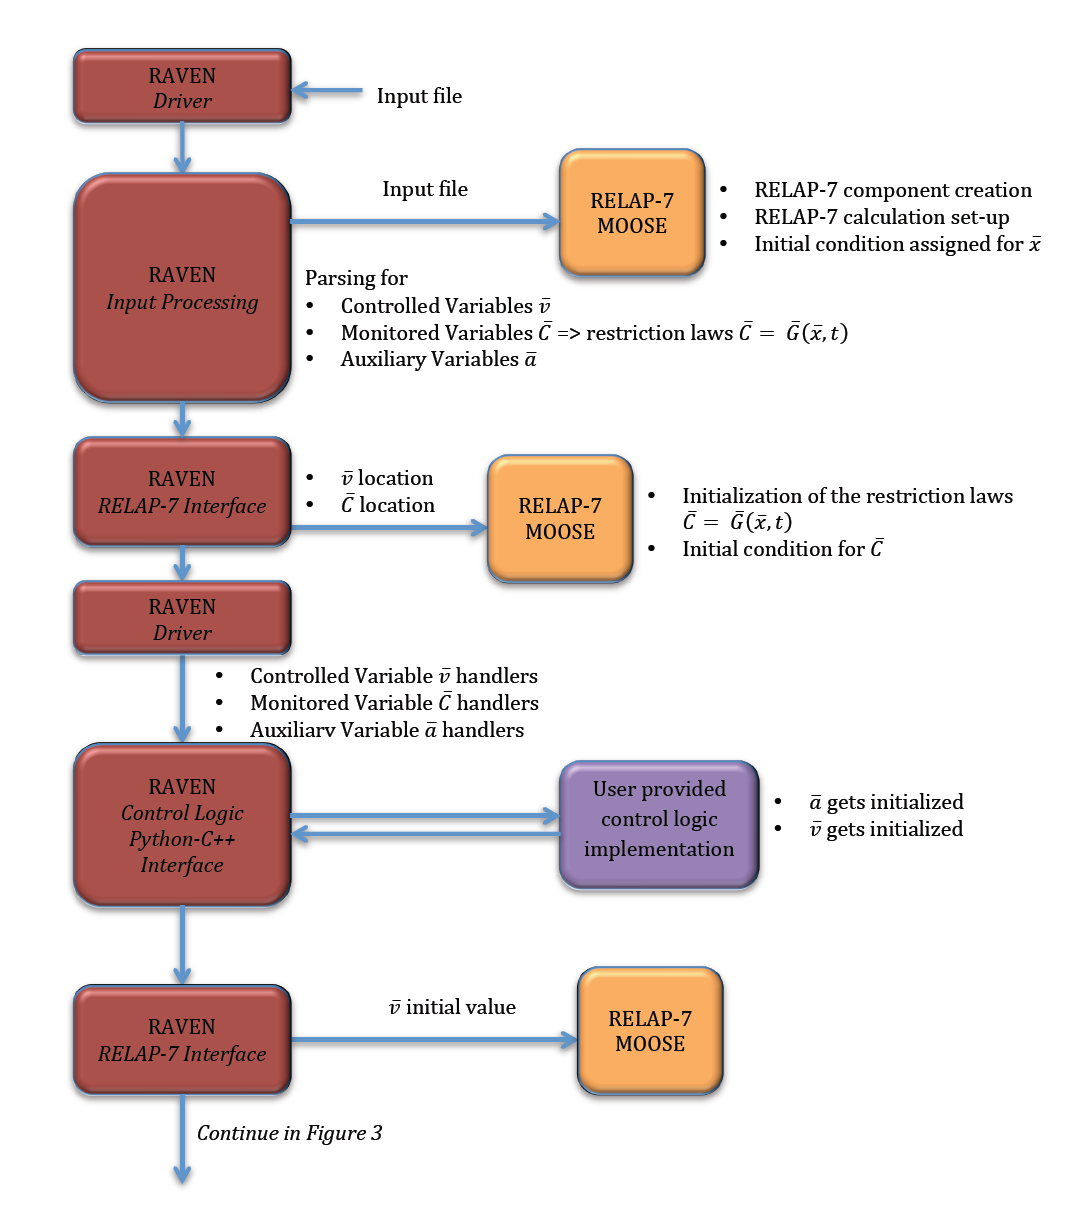
\includegraphics[width=0.8\textwidth]{figures/CalculationFlow_part_1.PNG}
  \caption{Control System Software Layout.}
  \label{fig:CalcFlow1}
\end{figure}

\begin{figure}[h] 
  \centering
     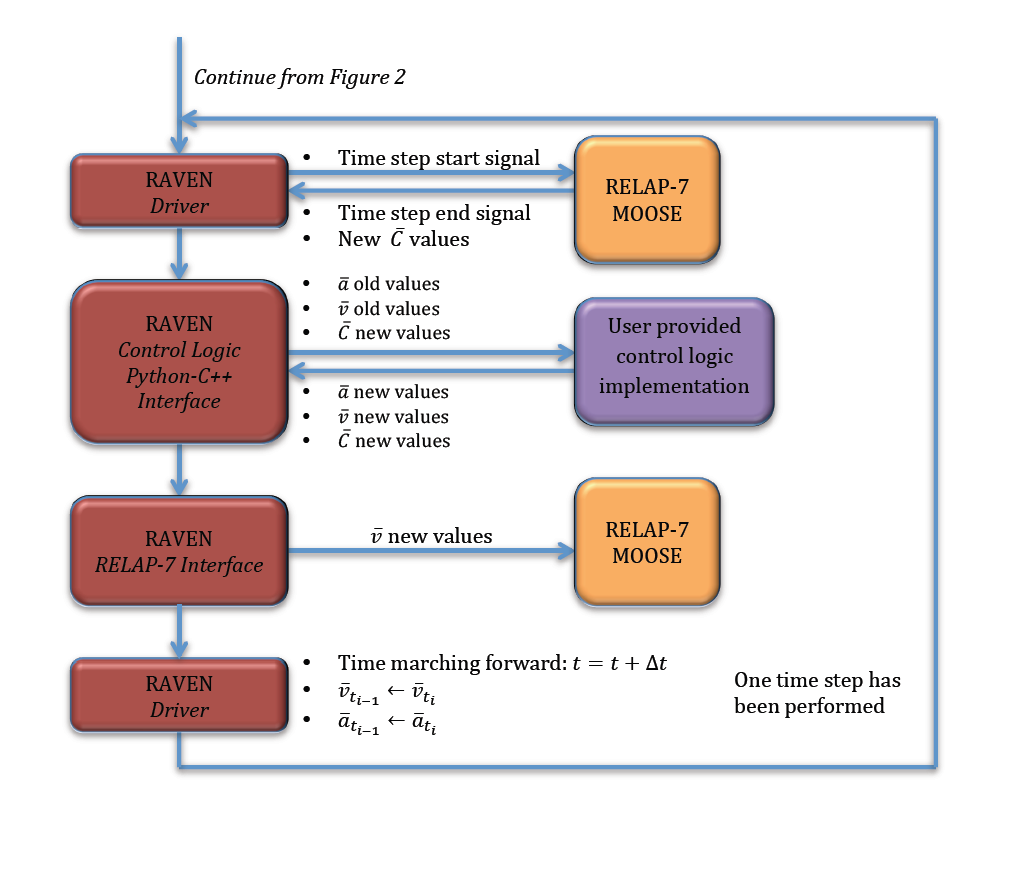
\includegraphics[width=0.8\textwidth]{figures/CalculationFlow_part_2.PNG}
  \caption{Control System Software Layout.}
  \label{fig:CalcFlow2}
\end{figure}

%%%%%%%%%%%%%%%%%%%%%%%%
\Section{PROBABILISTIC RISCK ASSESMENT DEMO} 
%%%%%%%%%%%%%%%%%%%%%%%%

%%%%%%%%%%%%%%%%%%%%%%%%%%%%%%
\Subsection{Tree miles island station black out} 
%%%%%%%%%%%%%%%%%%%%%%%%%%%%%%

%%%%%%%%%%%%%%%%%%%%%%%%%%%%%%
\Subsection{Resutls} 
%%%%%%%%%%%%%%%%%%%%%%%%%%%%%%

%%%%%%%%%%%%%%%%%
\Section{CONCLUSIONS}
%%%%%%%%%%%%%%%%%
Fin!


%\Section*{REFERENCES}
\setlength{\baselineskip}{12pt}
\begin{thebibliography}{300}
\bibitem{journal} B. Author(s), ``Title,'' {\it Journal Name in Italic}, 
          {\bf Volume in Bold}, pp. 34-89 (19xx).
\bibitem{proc_paper} C. D. Author(s), ``Article Title,'' {\it Proceedings of
          Meeting in Italic}, Location, Dates of Meeting, Vol. n, pp. 134-156 
          (19xx).
\bibitem{book} E. F. Author, {\it Book Title in Italic}, Publisher, City \&
          Country (19xx). 
\bibitem{website} ``Spallation Neutron Source: The next-generation 
          neutron-scattering facility in the United States,'' 
          http://www.sns.gov/documentation/sns\_brochure.pdf (2002).
\end{thebibliography}

\end{document}


